% Part: sets-functions-relations
% Chapter: relations
% Section: graphs

\documentclass[../../../include/open-logic-section]{subfiles}

\begin{document}

\olfileid{sfr}{rel}{grp}
\olsection{આલેખો}

\emph{આલેખ} એવી આકૃતિ છે જેમાં બિંદુઓને—જેને “ગાંઠો” અથવા
“શિરોબિંદુઓ” કહે છે—ધારો વડે જોડવામાં આવે છે.
આલેખો વિવિક્ત ગણિત અને સંગણકવિજ્ઞાનમાં સર્વત્ર વપરાતું સાધન છે.
વિવિધ પ્રકારનાં જાળાં જેવી મૂર્ત બાબતોથી માંડીને નિર્ણયોના
સંભવિત પરિણામો જેવાં અમૂર્ત માળખાં સુધી, સંબંધો અને માળખાંને
રજૂ કરવામાં અને દૃશ્યમાન કરવામાં તે અત્યંત ઉપયોગી છે.
સાહિત્યમાં ઘણા જુદા પ્રકારના આલેખો મળે છે; દાખલા તરીકે,
ધારો દિશાયુક્ત છે કે નહીં, તેમને લેબલ છે કે નહીં, કોઈ ગાંઠથી
તે જ ગાંઠ સુધી ધાર હોઈ શકે કે નહીં, એ જ ગાંઠો વચ્ચે એક કરતાં
વધુ ધારો હોઈ શકે કે નહીં, વગેરે બાબતોમાં તે જુદા પડે છે.
\emph{દિશાયુક્ત આલેખો}નું સંબંધો સાથે ખાસ જોડાણ છે.

\begin{defn}[દિશાયુક્ત આલેખ]
\emph{દિશાયુક્ત આલેખ} $G = \tuple{V, E}$ એ
\emph{શિરોબિંદુઓ}નો ગણ $V$ અને \emph{ધારો}નો ગણ
$E \subseteq V^2$ છે.
\end{defn}

\begin{explain}
આપણી વ્યાખ્યા મુજબ, આલેખ એટલે એક ગણ અને તેની પરનો એક સંબંધ.
અલબત્ત, આલેખોની વાત કરતી વખતે તેમને આકૃતિમાં દર્શાવવાની
અપેક્ષા સ્વાભાવિક છે: બે શિરોબિંદુઓ $v_1$ અને $v_2$ને
તીર વડે જોડીને આલેખ દોરી શકીએ, જો અને ફક્ત જો
$\tuple{v_1, v_2} \in E$. માત્ર સંબંધ અને આલેખ વચ્ચે
એક જ તફાવત છે: આલેખમાં શિરોબિંદુઓનો ગણ સ્પષ્ટ કરવામાં આવે છે,
એટલે કે, આલેખમાં છૂટાં શિરોબિંદુઓ હોઈ શકે છે.
જોકે મહત્વની વાત એ છે કે ગણ $X$ પરના દરેક સંબંધ $R$ને
દિશાયુક્ત આલેખ $\tuple{X, R}$ તરીકે જોઈ શકાય છે અને,
ઊલટું, દિશાયુક્ત આલેખ $\tuple{V, E}$ને
$E \subseteq V^2$ એવા સંબંધ તરીકે જોઈ શકાય છે,
જેમાં ગણ $V$ સ્પષ્ટપણે નિર્દિષ્ટ છે.
\end{explain}

\begin{ex}
$V = \{1, 2, 3, 4\}$ અને
$E = \{\tuple{1,1}, \allowbreak \tuple{1, 2}, \allowbreak \tuple{1, 3},
\allowbreak \tuple{2, 3}\}$ ધરાવતો આલેખ $\tuple{V, E}$
આવો દેખાય છે:
\begin{align*}
& 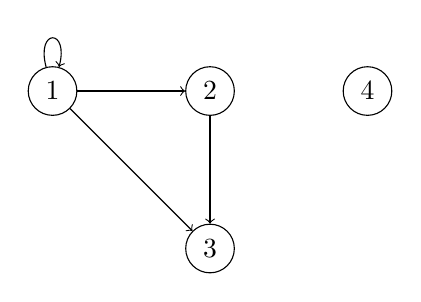
\begin{tikzpicture}[->,node distance=2cm]
  \node[draw,circle] (A) {$1$};
  \node[draw,circle] (B) [right of=A] {$2$};
  \node[draw,circle] (C) [below of=B] {$3$};
  \node[draw,circle] (D) [right of=B] {$4$};
  \draw (A) to [loop above]  (A);
  \draw (A) to  (B);
  \draw (A) to  (C);
  \draw (B) to  (C);
  \end{tikzpicture}
\intertext{આ આલેખ $\tuple{V', E}$થી જુદો છે,
  જેમાં $V' = \{1, 2, 3\}$ છે અને જે આવો દેખાય છે:}
& 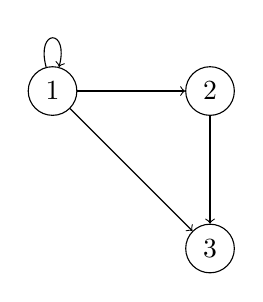
\begin{tikzpicture}[->,node distance=2cm]
  \node[draw,circle] (A) {$1$};
  \node[draw,circle] (B) [right of=A] {$2$};
  \node[draw,circle] (C) [below of=B] {$3$};
  \draw (A) to [loop above]  (A);
  \draw (A) to  (B);
  \draw (A) to  (C);
  \draw (B) to  (C);
  \end{tikzpicture}
\end{align*}
\end{ex}

\begin{prob}
  ગણ $\{1, 2, 3, 4\}$ પરના કરતાં-નાનું-અથવા-સમાન
  સંબંધ $\le$ને આલેખ તરીકે લો અને તેને અનુરૂપ આકૃતિ દોરો.
\end{prob}

\end{document}
